\documentclass{article}

\usepackage{amsthm}
\usepackage{amsfonts}
\usepackage{amsmath}
\usepackage{amssymb}
\usepackage{fullpage}
\usepackage{graphicx}
\usepackage[usenames]{color}
\usepackage{hyperref}
  \hypersetup{
    colorlinks = true,
    urlcolor = blue,       % color of external links using \href
    linkcolor= blue,       % color of internal links 
    citecolor= blue,       % color of links to bibliography
    filecolor= blue,        % color of file links
    }
    
\usepackage{listings}

\definecolor{dkdkgreen}{rgb}{0,0.4,0}
\definecolor{dkgreen}{rgb}{0,0.6,0}
\definecolor{gray}{rgb}{0.5,0.5,0.5}
\definecolor{mauve}{rgb}{0.58,0,0.82}
\definecolor{mPurple}{rgb}{0.58,0,0.82}
\definecolor{mGreen}{rgb}{0,0.6,0}
\definecolor{red}{rgb}{1,0,0}
\definecolor{orange}{rgb}{1,0.4,0}
\definecolor{burgandy}{rgb}{0.9,0.2,0}
\definecolor{dkred}{rgb}{0.6,0,0}

\lstdefinestyle{HaskellStyle}{
  frame=tb,
  language=haskell,
  aboveskip=3mm,
  belowskip=3mm,
  showstringspaces=false,
  columns=flexible,
  basicstyle={\small\ttfamily},
  numbers=none,
  numberstyle=\tiny\color{gray},
  keywordstyle=\color{blue},
  commentstyle=\color{dkgreen},
  stringstyle=\color{mauve},
  breaklines=true,
  breakatwhitespace=true,
  tabsize=3
}

\lstdefinestyle{CStyle}{
  frame=tb,
  language=C,
  aboveskip=3mm,
  belowskip=3mm,
  showstringspaces=false,
  columns=flexible,
  basicstyle={\small\ttfamily},
  numbers=none,
  numberstyle=\tiny\color{gray},
  keywordstyle=\color{blue},
  commentstyle=\color{red},
  stringstyle=\color{mauve},
  breaklines=true,
  breakatwhitespace=true,
  tabsize=3
}

\lstdefinestyle{WasmStyle}{
  frame=tb,
  language={[x86masm]Assembler},
  aboveskip=3mm,
  belowskip=3mm,
  showstringspaces=false,
  columns=flexible,
  basicstyle={\small\ttfamily},
  numbers=none,
  numberstyle=\tiny\color{gray},
  keywordstyle=\color{dkdkgreen},
  commentstyle=\color{mauve},
  stringstyle=\color{dkgreen},
  breaklines=true,
  breakatwhitespace=true,
  tabsize=3
}

\lstdefinestyle{AsmStyle}{
  frame=tb,
  language={[x86masm]Assembler},
  aboveskip=3mm,
  belowskip=3mm,
  showstringspaces=false,
  columns=flexible,
  basicstyle={\small\ttfamily},
  numbers=none,
  numberstyle=\tiny\color{gray},
  keywordstyle=\color{dkred},
  commentstyle=\color{burgandy},
  stringstyle=\color{mauve},
  breaklines=true,
  breakatwhitespace=true,
  tabsize=3
}

\lstset{frame=tb,
  language=haskell,
  aboveskip=3mm,
  belowskip=3mm,
  showstringspaces=false,
  columns=flexible,
  basicstyle={\small\ttfamily},
  numbers=none,
  numberstyle=\tiny\color{gray},
  keywordstyle=\color{blue},
  commentstyle=\color{dkgreen},
  stringstyle=\color{mauve},
  breaklines=true,
  breakatwhitespace=true,
  tabsize=3
}

\theoremstyle{theorem} 
   \newtheorem{theorem}{Theorem}[section]
   \newtheorem{corollary}[theorem]{Corollary}
   \newtheorem{lemma}[theorem]{Lemma}
   \newtheorem{proposition}[theorem]{Proposition}
\theoremstyle{definition}
   \newtheorem{definition}[theorem]{Definition}
   \newtheorem{example}[theorem]{Example}
\theoremstyle{remark}    
  \newtheorem{remark}[theorem]{Remark}


\title{CPSC-402 Report\\Compiler Construction}
\author{Scott Fitzpatrick  \\ Chapman University}

\date{\today}

\begin{document}

\maketitle

\begin{abstract}

\end{abstract}

\tableofcontents


\section{Introduction}\label{intro}
\medskip
This report contains the homework from Chapman University's 2022 Compiler Construction course (CPSC 402) and a project that studies the gcc compiler by comparing it to C++ code and WebAssembly.

\section{Homework}\label{homework}

\subsection{Week 1}

\noindent
Exercise 2.2.4: Give DFA's accepting the following languages over the alphabet $\{0,1\}$:

\medskip\noindent
b) The set of all strings with three consecutive 0's (not necessarily at the end)

\begin{center}
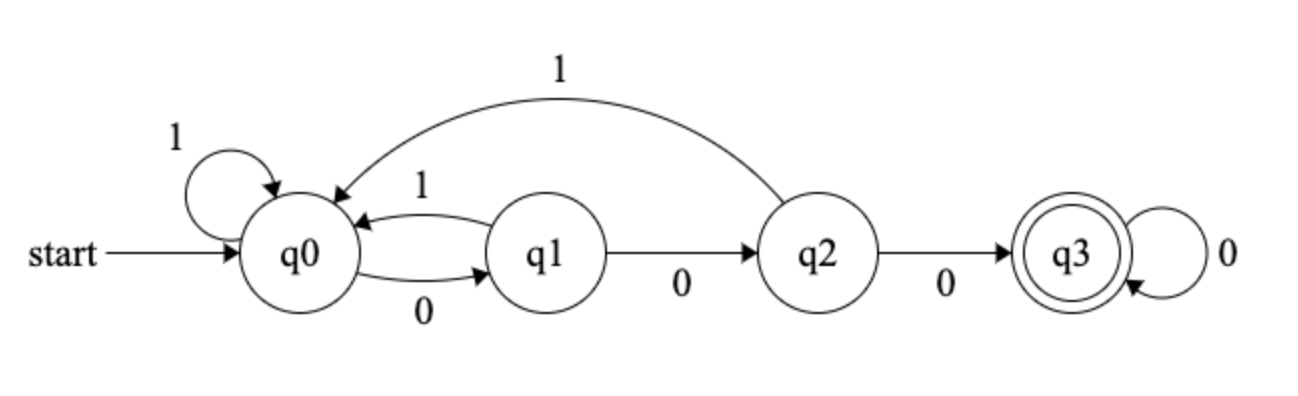
\includegraphics[width=0.75\textwidth]{Images/2.4.4b.png}
\end{center}

\medskip\noindent
c) The set of strings with 011 as a substring

\begin{center}
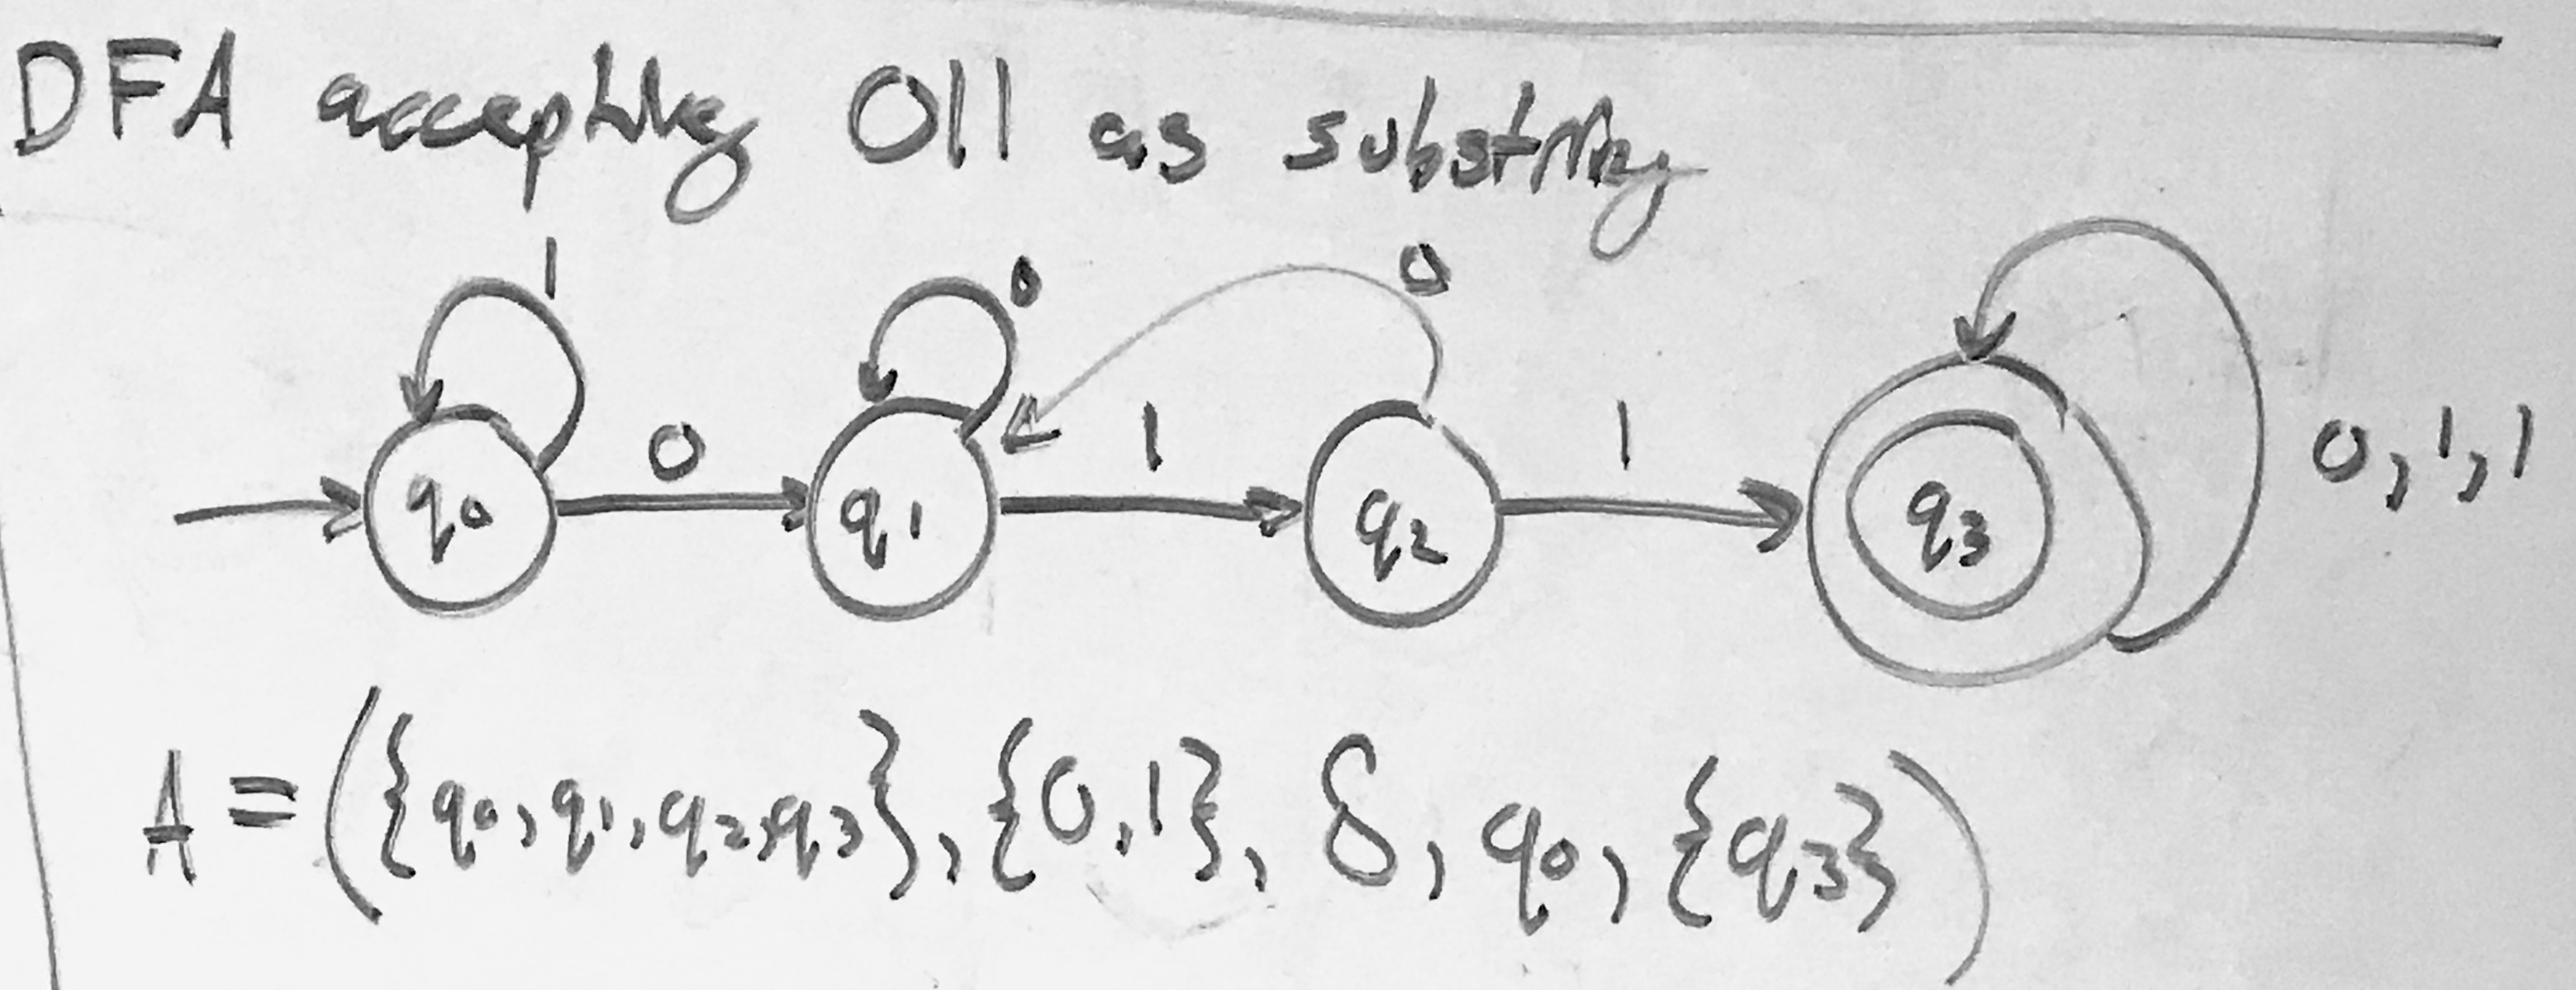
\includegraphics[width=0.75\textwidth]{Images/2.4.4c.png}
\end{center}


\subsection{Week 2}

\noindent
Exercise 2.3.4:

\medskip\noindent
a) The set of strings over alphabet $\{0,1,..., 9\}$ such that the final digit has appeared before.

\bigskip
\begin{center}
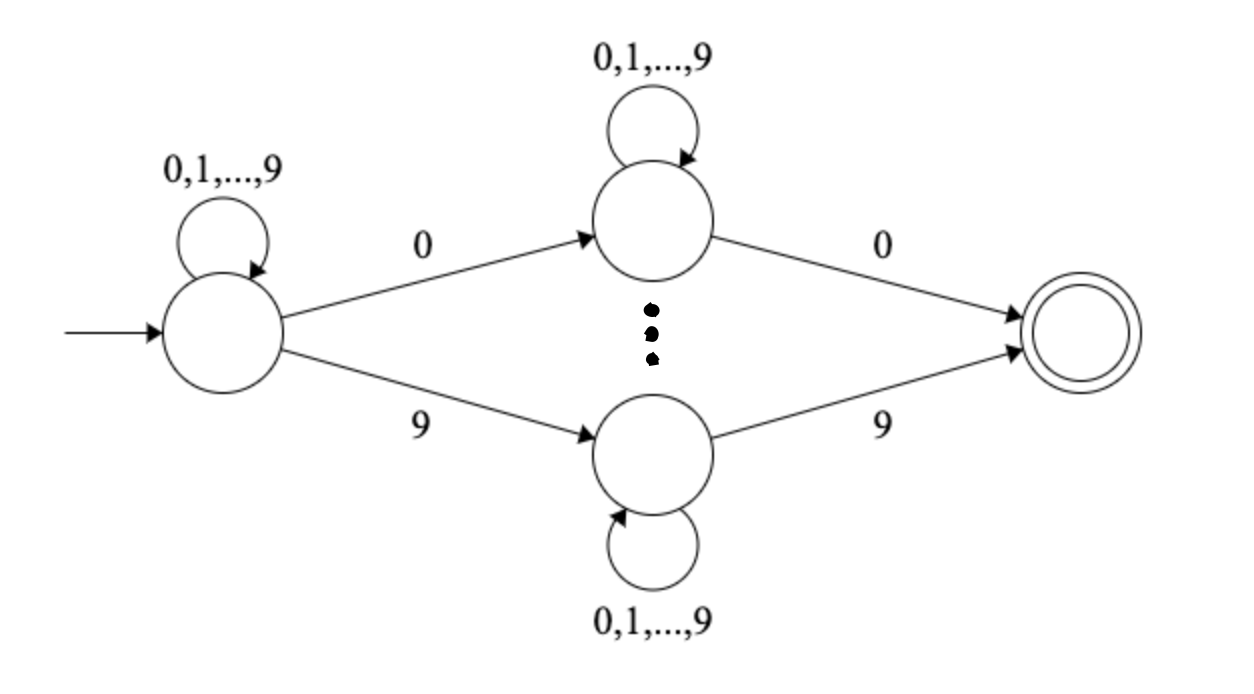
\includegraphics[width=0.55\textwidth]{Images/2.3.4a.png}
\end{center}

\medskip\noindent
b) The set of strings over alphabet $\{0,1,...,9\}$ such that the final digit has not appeared before.

\medskip
\begin{center}
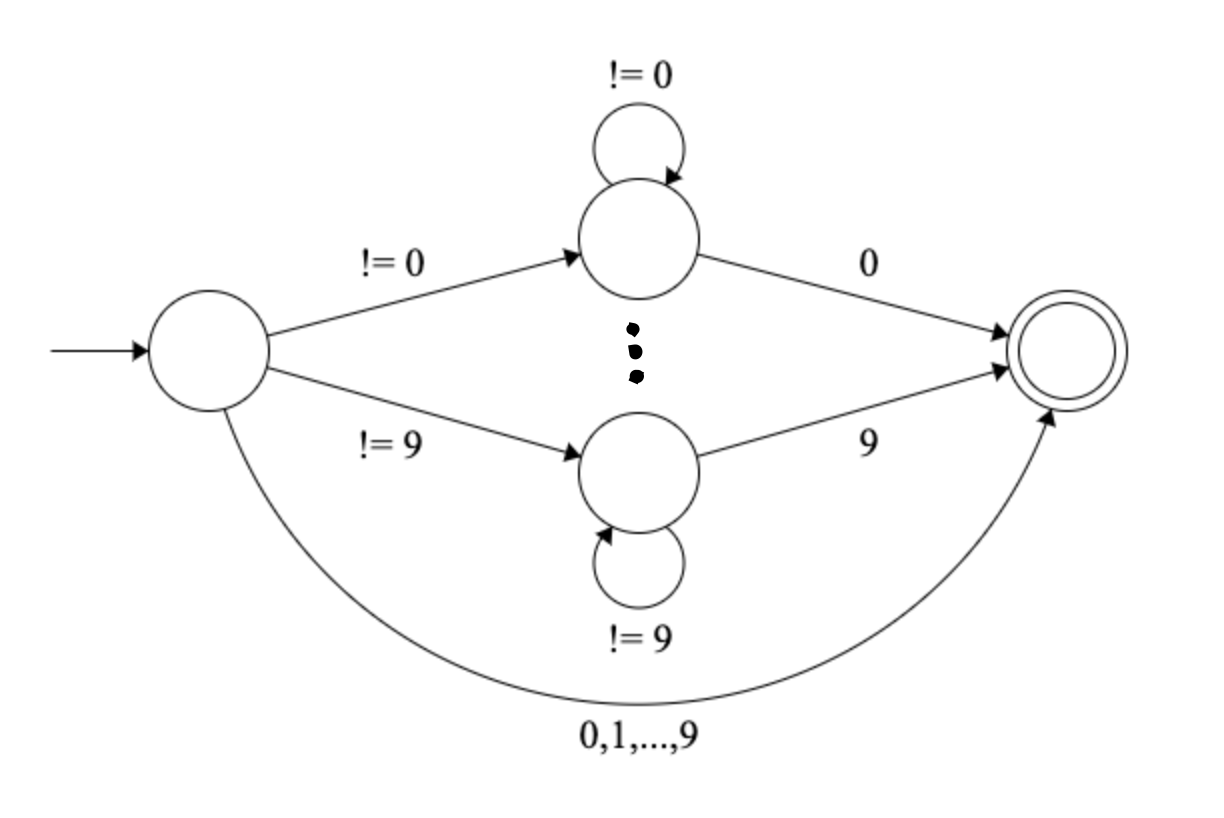
\includegraphics[width=0.55\textwidth]{Images/2.3.4b.png}
\end{center}

\medskip\noindent
c) The set of strings of $0$'s and $1$'s such that there are two $0$'s separated by a number of positions that is a number of $4$. Note that $0$ is an allowable multiple of $4$.

\medskip
\begin{center}
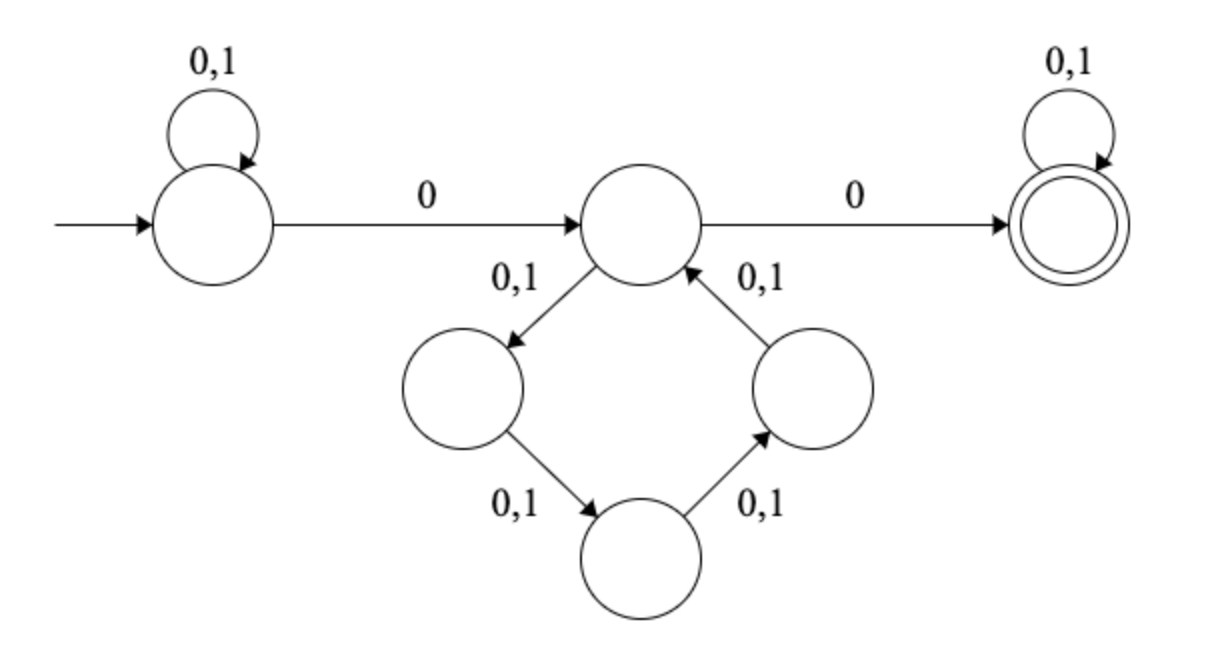
\includegraphics[width=0.55\textwidth]{Images/2.3.4c.png}
\end{center}

\medskip\noindent
Exercise 2.5.3:

\medskip\noindent
a) The set of strings consisting of zero or more a's followed by zero or more $b$'s, followed by zero or $c$'s.

\smallskip
\begin{center}
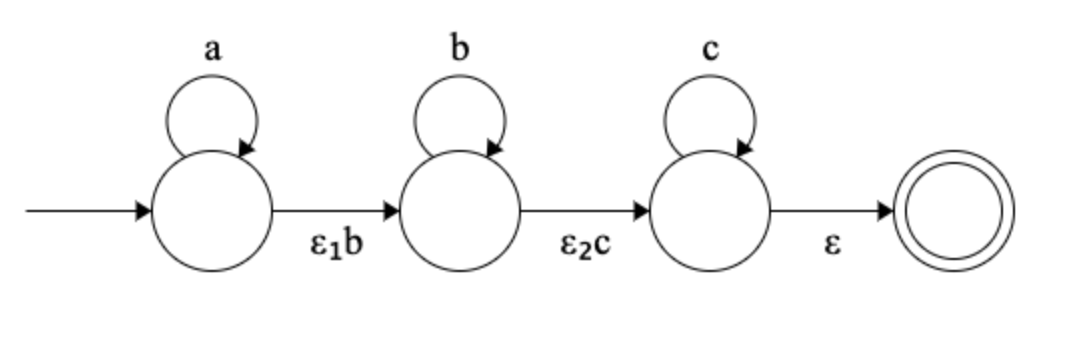
\includegraphics[width=0.75\textwidth]{Images/2.5.3a.png}
\end{center}

\medskip\noindent
b) The set of strings that consist of either $01$ repeated one or more times or $010$ repeated one or more times.

\medskip
\begin{center}
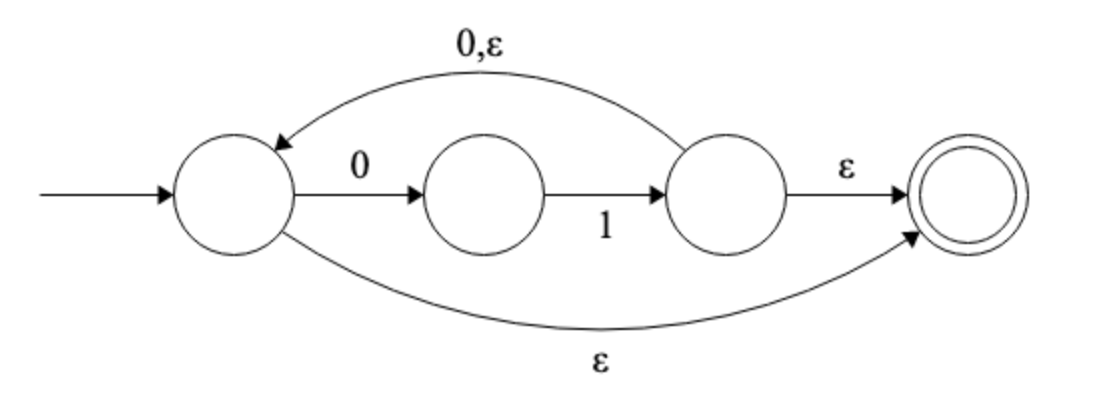
\includegraphics[width=0.75\textwidth]{Images/2.5.3b.png}
\end{center}

\medskip\noindent
c) The set of strings of $0$'s and $1$'s such that at least one of the last ten positions is a $1$.

\medskip
\begin{center}
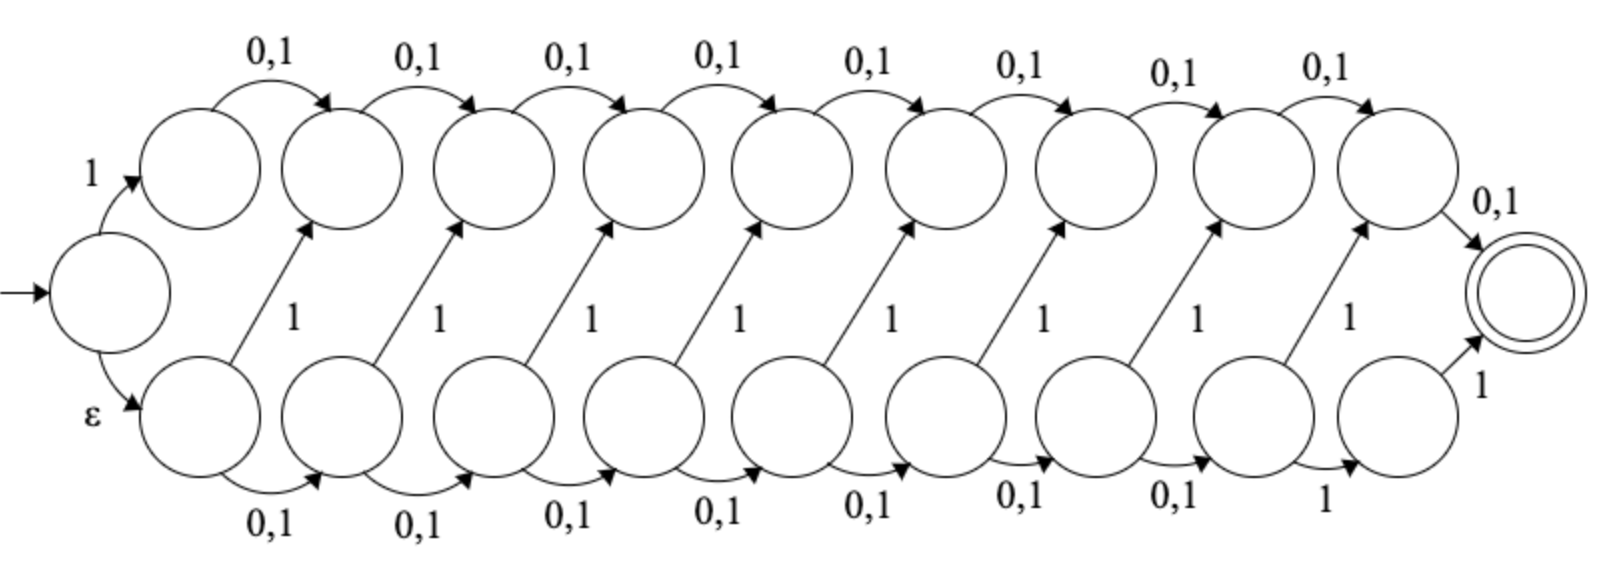
\includegraphics[width=0.75\textwidth]{Images/2.5.3c.png}
\end{center}


\subsection{Week 3}

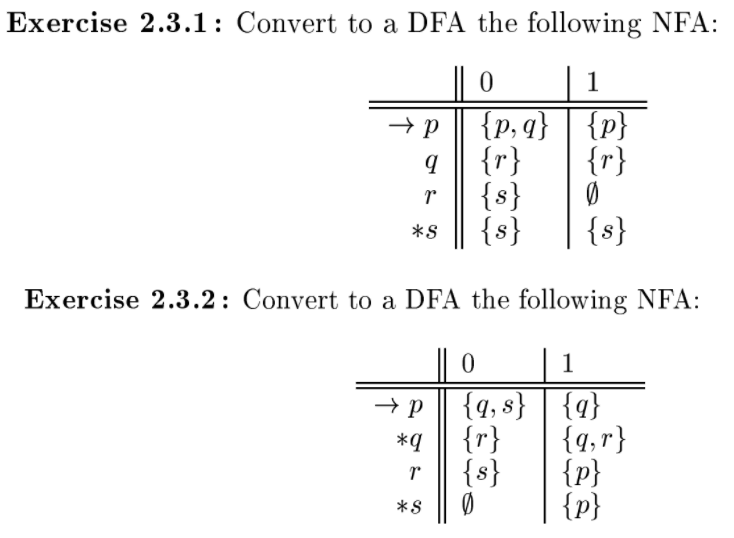
\includegraphics[width=0.65\textwidth]{Images/2.3.1and2.3.2_chart.png}

\noindent
The following DFA's above can be drawn as:

\medskip
\begin{center}
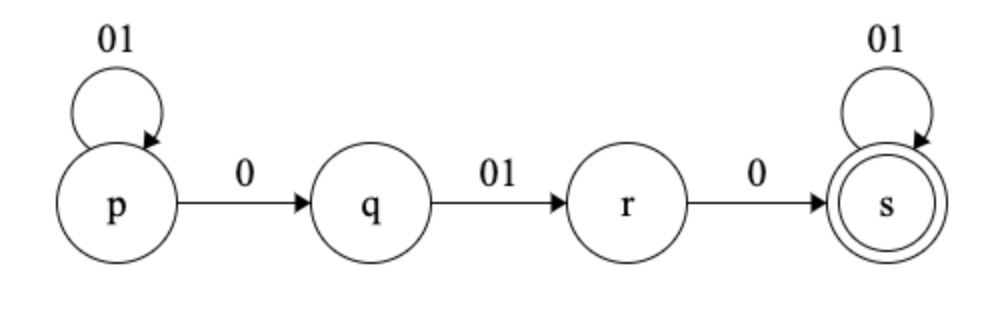
\includegraphics[width=0.50\textwidth]{Images/2.3.1.png}

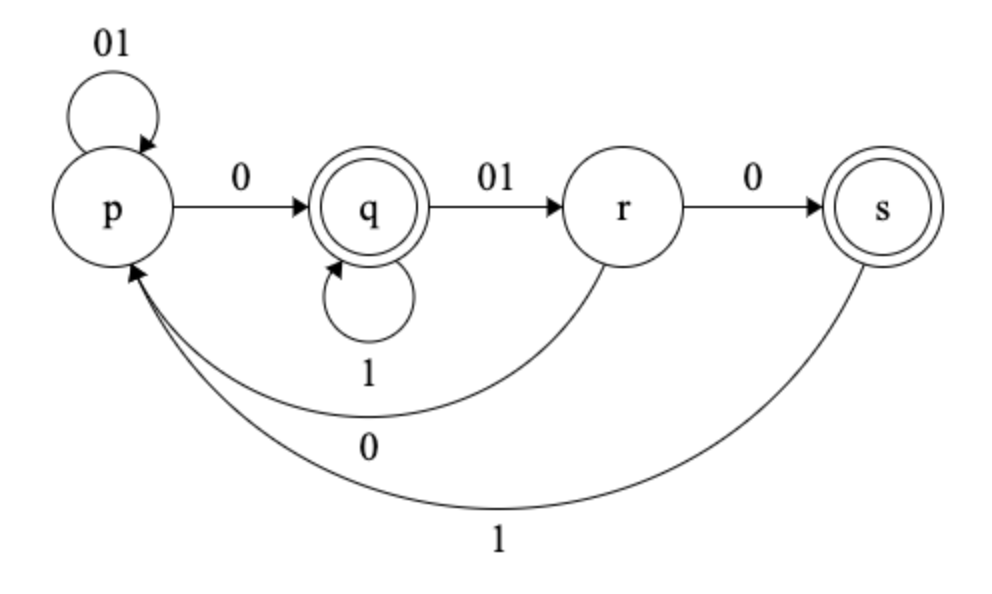
\includegraphics[width=0.50\textwidth]{Images/2.3.2.png}
\end{center}

\medskip\noindent
In order to convert a dfa to an nfa, there can be only one final state. The initial state can remain the same, but the automata must result in one final state every time. Therefore, "final" should not return a set but instead a state.

\begin{lstlisting}[style=HaskellStyle]
    -- convert an NFA to a DFA
    nfa2dfa :: NFA s -> DFA [s]
    nfa2dfa nfa = DFA {
    -- exercise: correct the next three definitions 
    dfa_initial = [nfa_initial nfa],
    dfa_final = let final qs = disjunction (map(nfa_final nfa) qs) in final,
    dfa_delta = let
        f [] c = []
        f (q:qs) c = concat [nfa_delta nfa q c, f qs c] in f }
\end{lstlisting}

\subsection{Week 4}
\label{sec:week4}

\medskip\noindent
\begin{lstlisting}[style=CStyle]
    // a fibonacci function showing most features of the C-- language

    int mx () {
        return 5000000 ;
    }

    int main () {
        int lo ; 
        int hi ;
        lo = 1 ;
        hi = lo ;
        printf("%d",lo) ;
        while (hi &lt; mx()) {
            printf("%d",hi) ;
            hi = lo + hi ;
            lo = hi - lo ;
        }
        return 0 ;
    }
\end{lstlisting}

\medskip\noindent
This is the parse tree (concrete syntax tree) for the C$--$ code listed above:

\medskip\noindent
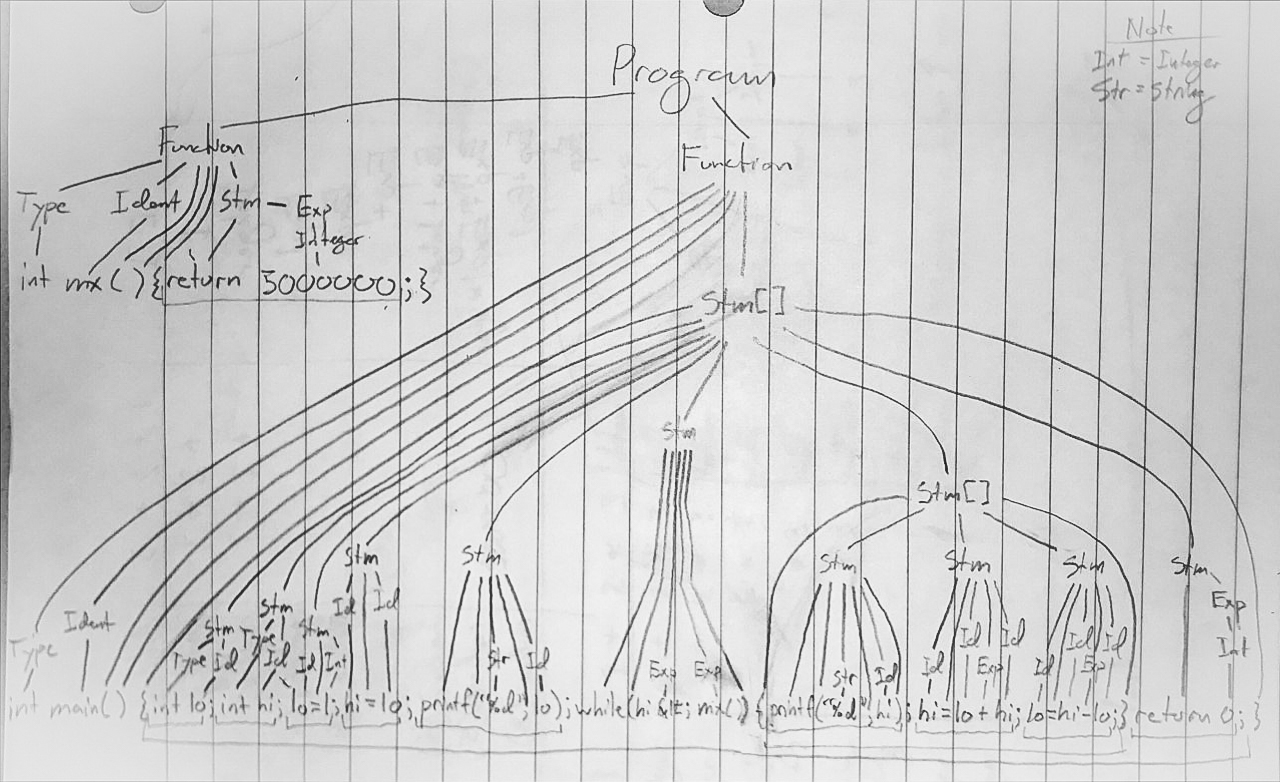
\includegraphics[width=1\textwidth]{Images/ConcreteSyntaxTree.jpg}

\medskip\noindent
Here is the respective abstract syntax tree:

\medskip\noindent
\begin{center}
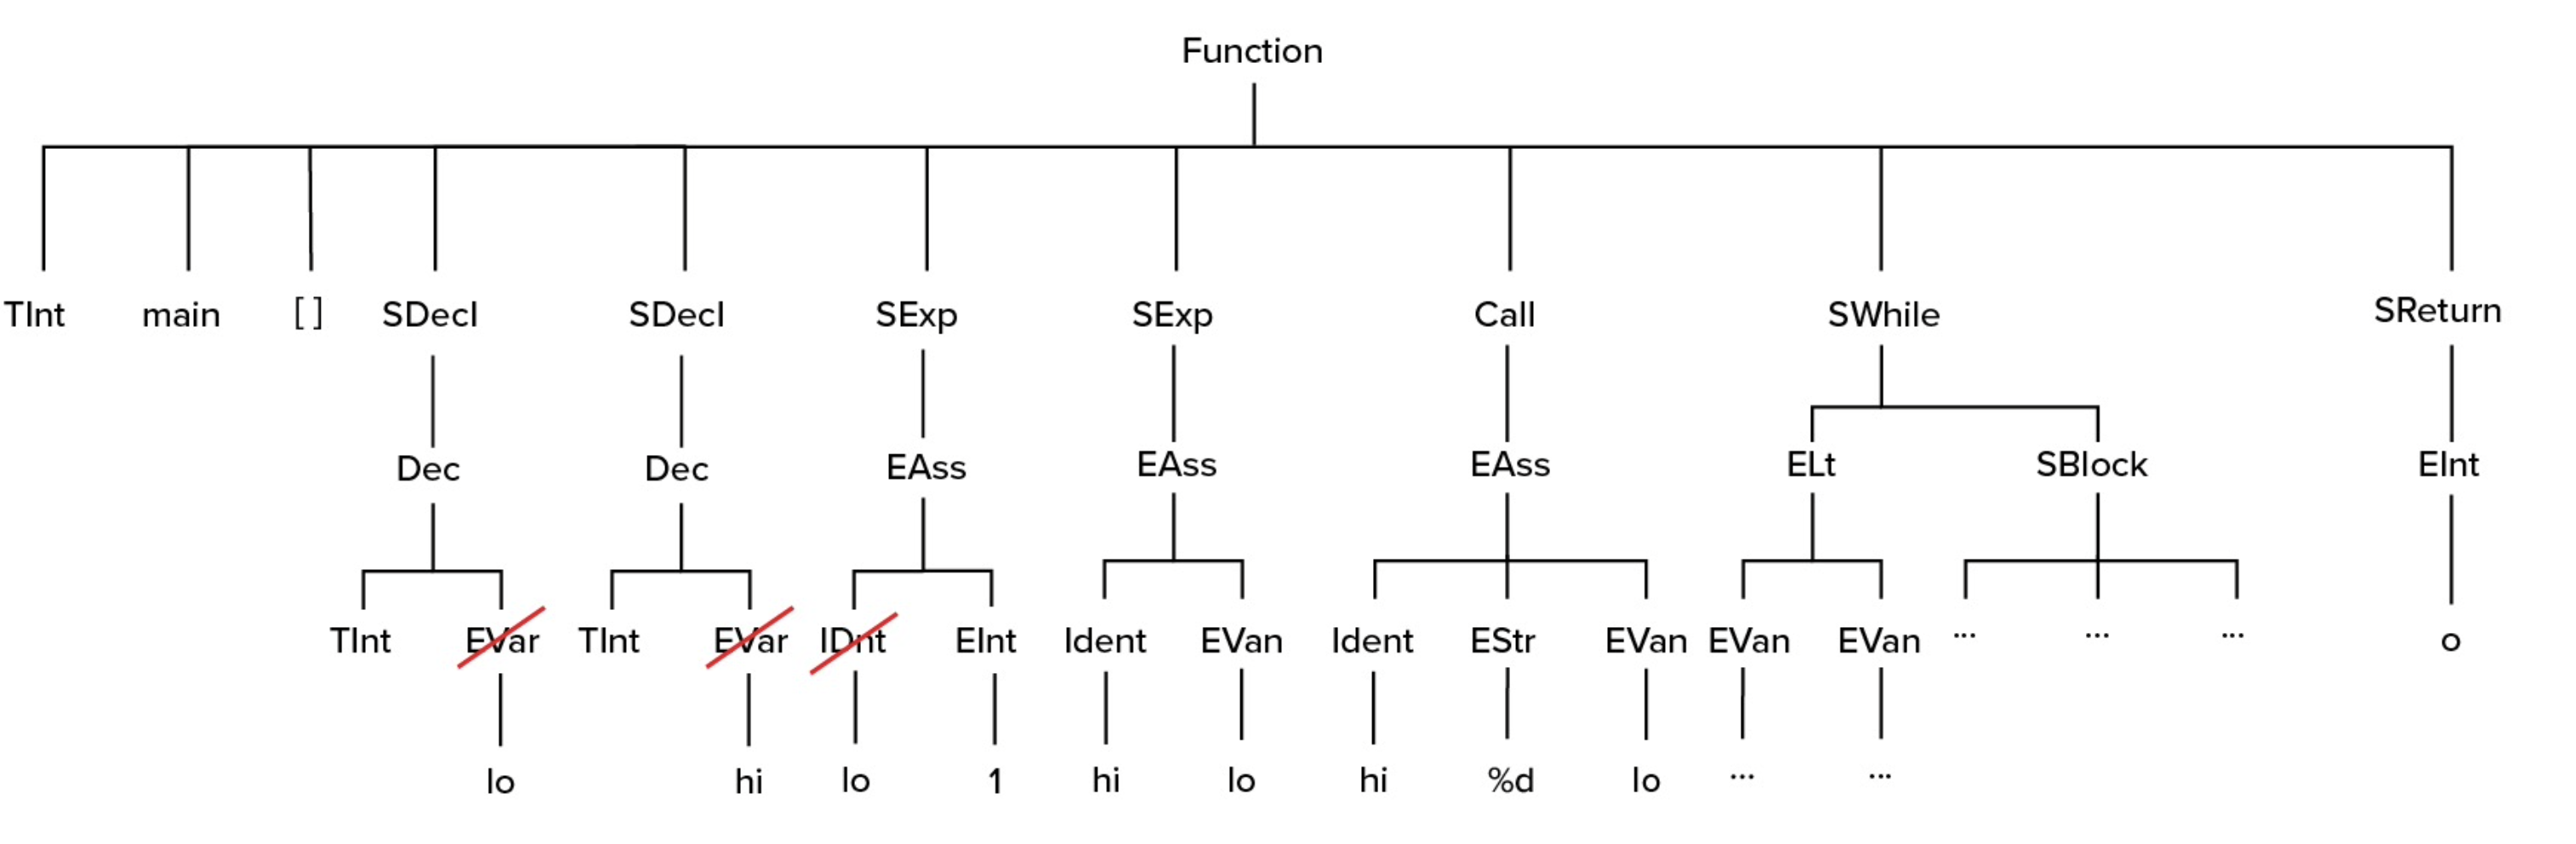
\includegraphics[width=0.98\textwidth]{Images/fib_ast.png}
\end{center}


\section{Project}
\medskip\noindent
This portion of the report will explain compiled code from WebAssembly and the gcc (x86-64 12.1) compiler in depth. We will cover topics such as the stack, abstract syntax, and the key differences between WebAssembly and Assembly These example programs will be compiled and explained in detail using the same workflow used in \href{https://github.com/sfitzpatrickchapman/CPSC_402_Compiler_Construction/tree/main/Assignment4}{Assignment 4} and \href{https://godbolt.org/}{this compiler explorer}.

\subsection{Introduction}
We will take simple C++ programs and compile them to binary. Each program increases in complexity and contain simple math operations. The binary formats will be WebAssembly and x86 assembly.

\subsection{easy\_mult.cc}
To start simple, we will start with this C++ code:

\medskip\noindent
\begin{lstlisting}[style=CStyle]
    int main () {
        return 2*3;
    }
\end{lstlisting}

\medskip\noindent
This program returns $2*3$ within the main program. This may seem quite obvious, especially from the perspective of an experience programmer who does not usually have to think about the compilation process. However, much is actually going on underneath the hood in order to go from C++ to binary. Using node.js and the WebAssembly Binary Toolkit, we will generate a \verb|.wat| file which contains the respective WebAssembly to our \verb|easy_mult.cc| program. This generated \verb|.wat| file looks like this:

\medskip\noindent
\begin{lstlisting}[style=WasmStyle]
    (module
        (func
            $main               ; function name
            (result i32)        ; return type (32-bit integer)
            (i32.const 2)       ; 2
            (i32.const 3)       ; 3
            i32.mul             ; *
            return              ; return
        )
        (export "main" (func $main))
    )
\end{lstlisting}

\medskip\noindent
This may seem just slightly overwhelming at first, so let's quickly cover some of the basic code. The export line at the bottom will export our main function which is defined above it. The main function is denoted as: \verb|\$main|. \verb|result$ $i32| means that the function will return a 32-bit integer. Now we can focus on the logical code within the main function which is:

\medskip\noindent
\begin{lstlisting}[style=WasmStyle]
            (i32.const 2)
            (i32.const 3)
            i32.mul
\end{lstlisting}

\medskip\noindent
First, let's quickly review some simple syntax. In WebAssembly, the \verb|i32.const| mnemonic holds an integer value of 32 bits. Similarly, the \verb|i32.mul| mnemonic represents multiplication for integers. For the sake of simplicity, we can view them this way for now:

\medskip\noindent
\begin{lstlisting}[style=CStyle]
            2
            3
            *
\end{lstlisting}

\medskip\noindent
As you have noticed, this represents $2*3$. You may be wondering why these three WebAssembly lines are out of order though. If these lines were written chronologically as a math equation, it would appear to be: $(2$ $3$ $*)$. This is because a stack is used to compile and execute math equations in C++. So math operations are performed by pushing and popping values like these onto the stack. In order to properly push mathematical numbers and operators onto the stack, reverse polish notation (RPN) must be used. After the equation is fully pushed, it can be calculated as it is popped off the stack. Here is a visual of the RPN conversion and how it applies in the WebAssembly file:

\bigskip
\begin{center}
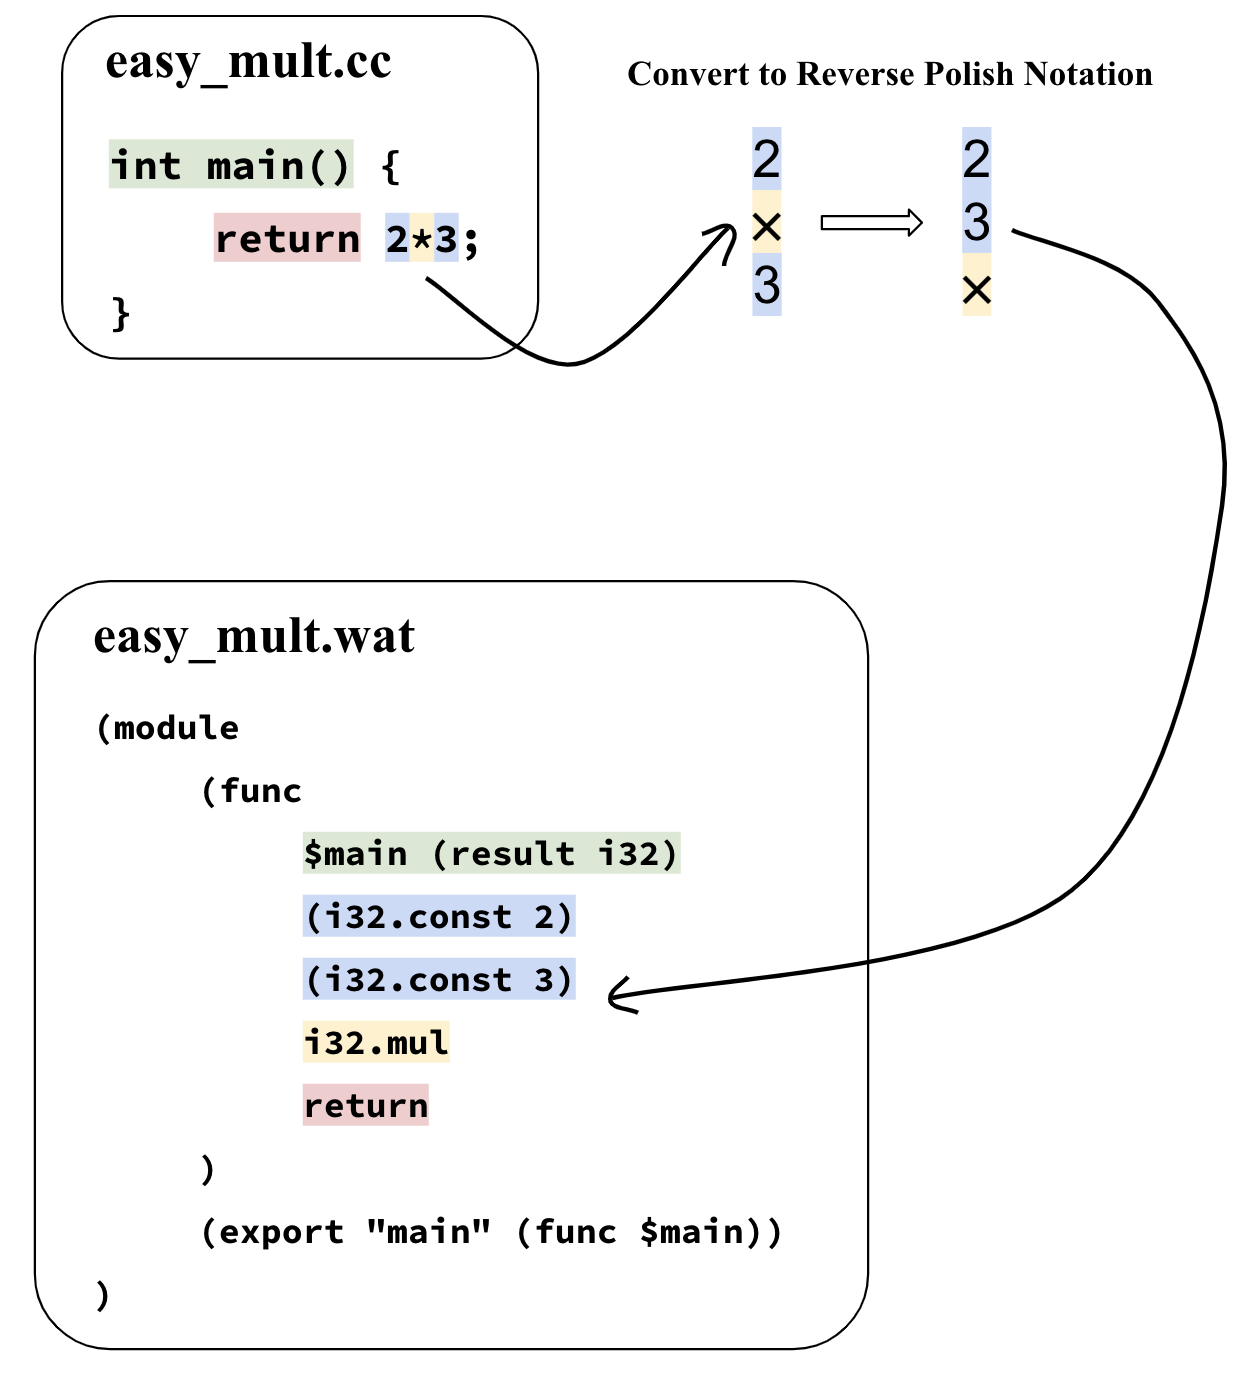
\includegraphics[width=0.55\textwidth]{Images/easy_mult_cc_to_wat.png}
\end{center}

\medskip\noindent
In the next example, we will view a more complex equation. For now, we will compare the WebAssembly to the assembly complied by the gcc compiler. With \verb|easy_mult.cc| inserted into \href{https://godbolt.org/}{this compiler explorer} with x86-64 12.1 selected, we get:

\medskip\noindent
\begin{lstlisting}[style=AsmStyle]
    main:
        push    rbp         ; push val of register onto stack
        mov     rbp, rsp    ; copy stack pointer val to base pointer
        mov     eax, 6      ; copy 6 to the eax register
        pop     rbp         ; cleanup
        ret                 ; cleanup
\end{lstlisting}

%https://blog.holbertonschool.com/hack-virtual-memory-stack-registers-assembly-code/
\medskip\noindent
There is much to digest here. When reading assembly, it is crucial to think about the stack and how each line effects it. Let's start by looking at \verb|push rbp|. This instruction pushes the value of the register, \verb|rbp| onto the stack. \verb|rbp| is the memory address of the base of the previous stack frame. This action will cause the value \verb|rsp| to be the memory address of the top of the stack. This next step is to copy the value of the stack pointer, \verb|rsp|, to the base pointer, \verb|rbp|. This is done with \verb|mov rbp, rsp| Now, \verb|rbp| and \verb|rsp| point to the top of the stack. Now we must copy the answer, 6, to the \verb|eax| register with: \verb|mov eax, 6|. Finally, the last two lines clean up the stack for it's next usage \cite{AC}.

\bigskip\noindent
\underline{\textbf{The Differences Between WebAssembly and Assembly}}

\medskip
It is also important to consider the differences between WebAssembly and assembly. Assembly language is a low-level programming language that bridges programming languages such as C++ to the computer hardware \cite{AL}. When compiling with gcc, we obtain a binary file. The file appears as assembly language which allows us to understand what is actually going on in the stack and how the program is actually working in terms of interacting with the computer hardware. The literal binary (1's and 0's) can also be written out by referencing the opcodes. WebAssembly is like a low-level assembly language in the aspect that it is a compiled binary file. However, it is built to run in modern web-browsers. It provides a way to run code written in a variety of languages on the web at near native speed. This allows users to run client applications on the web \cite{WA}. There are clearly some noticeable differences in syntax between assembly language and WebAssembly which we will go over in these three examples. You may notice that WebAssembly is much easier to read and this is because it is not specific to a certain type of processor, unlike the assembly language code that is generated with gcc in this report. We will continue to look at more assembly code when we compare easy\_mult.cc to a modified and more advanced version.


\subsection{easy\_mult\_var.cc}
\medskip\noindent
Now lets look at this code. It is the same as easy\_mult.cc, but it has a different equation and uses an integer variable, \verb|foobar|, to store it.

\medskip\noindent
\begin{lstlisting}[style=CStyle]
    int main () {
        int foobar = (2+3)*2;
        return foobar;
    }
\end{lstlisting}

\medskip\noindent
The respective WebAssembly code is:

\medskip\noindent
\begin{lstlisting}[style=WasmStyle]
    (module
        (func
            $main
            (result i32)
            (local $ifoobar$0 i32)          ; define local variable integer
            (i32.const 2)                   ; 2
            (i32.const 3)                   ; 3
            i32.add                         ; +
            (i32.const 2)                   ; 2
            i32.mul                         ; *
            (local.set $ifoobar$0)          ; set local variable integer
            (local.get $ifoobar$0)          ; get local variable integer
            return
        )
        (export "main" (func $main))
    )
\end{lstlisting}

\medskip\noindent
To keep things simple, we will again start by focusing on the equation.

\medskip\noindent
\begin{lstlisting}[style=WasmStyle]
            ...
            (i32.const 2)                   ; 2
            (i32.const 3)                   ; 3
            i32.add                         ; +
            (i32.const 2)                   ; 2
            i32.mul                         ; *
            ...
\end{lstlisting}

\medskip\noindent
As you can see, the RPN is the very similar to the previous C++ example. However, now it is important to consider the parentheses. Below, we can view the conversion from the original equation to the RPN equation. We can also see how the RPN equation eventually leads to the answer as values are popped from the stack from top down.

\medskip\noindent
\begin{lstlisting}[style=CStyle]
    (2                   2
     +                   3       5
     3)    -- to -->     +   =   2   =   10
     *                   2       *
     2                   *
\end{lstlisting}

\medskip\noindent
We will see that 10 is the correct value when we analyze the assembly code. Before we do this, we will go over the new WebAssembly code within this main function which is:

\medskip\noindent
\begin{lstlisting}[style=WasmStyle]
            ...
            (local $ifoobar$0 i32)          ; define local variable
            ...
            (local.set $ifoobar$0)          ; set local variable
            (local.get $ifoobar$0)          ; get local variable
            ...
\end{lstlisting}

\medskip\noindent
\verb|(local $ifoobar$0 i32)| creates a local variable for the register named foobar with a 32-bit integer value. This line pertains to our integer declaration of \verb|foobar|. The next line, \verb|(local.set $ifoobar$0)|, sets the value of \verb|foobar|. This is a result of initializing \verb|foobar| with the value of $(2+3)*2$ which equals $10$. Also, the \verb|$i| denotes that \verb|foobar| is an integer. Lastly, \verb|(local.get $ifoobar$0 i32)| gets the value from the register, allowing the local variable which is the integer value, $10$, to be returned.

\medskip\noindent
Let's again view the assembly code complied by the gcc compiler. Now we can also compare easy\_mult.cc and easy\_mult\_var.cc in this regard.

\medskip\noindent
\begin{lstlisting}[style=AsmStyle]
    main:
        push    rbp
        mov     rbp, rsp
        mov     DWORD PTR [rbp-4], 10
        mov     eax, DWORD PTR [rbp-4]
        pop     rbp
        ret
\end{lstlisting}

\medskip\noindent
If you compare this assembly code to \verb|easy_mult.cc|'s assembly code, you will notice that the only change is that \verb|mov| is on an additional line. This is because to declare/initialize \verb|foobar| as a local variable it must first be moved to a specific memory address, and then store the variable in a register. The two lines can be seen below:

\medskip\noindent
\begin{lstlisting}[style=AsmStyle]
        ...
        mov     DWORD PTR [rbp-4], 10       ; set memory at address [rbp-4] to 10
        mov     eax, DWORD PTR [rbp-4]      ; store address [rbp-4] in the register
        ...
\end{lstlisting}

\medskip\noindent
``\verb|mov DWORD PTR [rbp-4], 10|" sets the memory at address \verb|rbp-4| to 10. \verb|rbp-4| is where our iconic local variable, \verb|foobar| will be stored. we can also see that the stored value, $10$, is the correct output from our equation. The reason why ``foobar" isn't actually found in the assembly code is because the computer only needs the memory address on the stack instead of the actual variable name. The next line, \verb|mov eax, DWORD PTR [rbp-4]|, simply stores \verb|rbp-4| in the \verb|eax| register.

\bigskip\noindent
\underline{\textbf{Considering the Abstract Syntax Tree}}

\medskip
Abstract syntax trees (AST's) can be used to form main intermediate representations of the compiler's front-end (for both WebAssembly and assembly). For an example of an abstract syntax tree, see \hyperref[sec:week4]{Week 4} in the homework section. As you can see, AST's represent the grammatical structure of the parsed input. If you have noticed, there are no keywords or punctuation such as, \verb|(),;,else|, in AST's because at this point, the compiler only cares about the abstract structure \cite{AS}. The compiler uses recursion on the abstract syntax to generate the code found in our WebAssembly and assembly files. The branches and levels of abstract syntax within each tree correlate to the structure of assembly code. It is useful to think about this correlation when reviewing the assembly code.

\subsection{find\_avg.cc}
\medskip\noindent
Let's take a look at a less basic example. The following program also consists of a main function. However, it calls a function, \verb|findAverage()| to calculate the average of the given double values, $12.3$ and $27.5$. Lastly, main simply closes by returning the typical value of 0. Here is the C++ code:

\medskip\noindent
\begin{lstlisting}[style=CStyle]
    double findAverage(double a, double b) {
        double avg = (a+b)/2;
        return avg;
    }

    int main() {
        double myAvg;
        myAvg = findAverage(12.3, 27.5);

        return 0;
    }
\end{lstlisting}

\medskip\noindent
It is helpful to try to think about what the WebAssembly and assembly code may look like before looking at it. You would be correct to assume there would be a whole new function above the main function in both WebAssembly and assembly. Here is the respective WebAssembly code:

\medskip\noindent
\begin{lstlisting}[style=WasmStyle]
    (module
        (func
            $findAverage                ; function name
            (param $da$0 f64)           ; input type double
            (param $db$0 f64)           ; input type double
            (result f64)                ; return 64-bit double
            (local $davg$0 f64)         ; define local variable double
            (local.get $da$0)           ; get input a
            (local.get $db$0)           ; get input b
            f64.add                     ; add 64-bit doubles
            (i32.const 2)               ; 2 (integer)
            f64.div                     ; divide 64-bit
            (local.set $davg$0)         ; set avg
            (local.get $davg$0)         ; get avg
            return                      ; return
        )
        (func
            $main                       ; function name
            (result i32)                ; return 32-bit integer
            (local $dmyAvg$0 f64)       ; define local variable double
            (f64.const 12.3)            ; 12.3 (double)
            (f64.const 27.5)            ; 27.5 (double)
            (call $findAverage)         ; call findAverage function
            (local.set $dmyAvg$0)       ; set myAvg
            (i32.const 0)               ; 0 (integer)
            return                      ; return
        )
        (export "main" (func $main))
    )
\end{lstlisting}

\medskip\noindent
Some of the primary differences in AssemblyLanguage code from this example from the last, are the usage of \verb|param|, \verb|f64|, and \verb|call|. \verb|param|, which can be found in the 2nd and 3rd lines of \verb|$findAverage|, are simply the input parameters for the function. In this case, they input 12.3 and 27.5. In those same lines, we can see that there is now \verb|f64|, which is different from \verb|easy_mult_var| which used \verb|i32|. This is because \verb|f64| is capable of storing 64-bit double values unlike \verb|i32| which does not have enough space. \verb|f64| can be found on a variety of other lines where 64-bit doubles are required. Lastly, We should take a look at \verb|(call $findAverage)| in \verb|$main|. This simply is WebAssembly's way of calling a function and is using the provided constant double value on the line above. Furthermore, \verb|func $findAverage| contains the math two add two inputted double values which is later returned as a type double. We can again see the Reverse Polish Notation (RPN):

\medskip\noindent
\begin{lstlisting}[style=WasmStyle]
            ...
            (local.get $da$0)           ; a
            (local.get $db$0)           ; b
            f64.add                     ; +
            (i32.const 2)               ; 2
            f64.div                     ; /
            ...
\end{lstlisting}

\medskip\noindent
This equation is very similar to \verb|easy_mult_var.cc|. It just uses division instead of multiplication with the purpose of finding an average.

\medskip\noindent
\begin{lstlisting}[style=CStyle]
    (a                   a
     +                   b      a+b
     b)    -- to -->     +   =   2   =   (a+b)/2
     /                   2       /
     2                   /
\end{lstlisting}

\medskip\noindent
Now we can move onto the assembly code version which should seem a bit more complicated. There is also a key below that contains the meanings of the register types, instruction types and more. Please view them on the next two pages.

\bigskip
\bigskip
\bigskip
\bigskip
\bigskip
\bigskip
\bigskip

\medskip\noindent
\begin{lstlisting}[style=AsmStyle]
    findAverage(double, double):
        push    rbp
        mov     rbp, rsp
        movsd   QWORD PTR [rbp-24], xmm0        ; set mem address ptr [rbp-24] to 64-bit double reg xmm0
        movsd   QWORD PTR [rbp-32], xmm1        ; set mem address ptr [rbp-32] to 64-bit double reg xmm1
        movsd   xmm0, QWORD PTR [rbp-24]        ; move ptr of first user input to reg xmm0
        addsd   xmm0, QWORD PTR [rbp-32]        ; w/ ptr, add 2nd user input to val at reg xmm0
        movsd   xmm1, QWORD PTR .LC0[rip]       ; move RIP-rel address ptr (str double-word)to reg xmm1
        divsd   xmm0, xmm1                      ; divide xmm0 val (39.8) by val xmm1 (2)
        movsd   QWORD PTR [rbp-8], xmm0         ; move mem address ptr [rbp-8] to reg xmm0
        movsd   xmm0, QWORD PTR [rbp-8]         ; move reg xmm0 to mem address ptr [rbp-8]
        movq    rax, xmm0                       ; move xmm0 val to rax register
        movq    xmm0, rax                       ; move rax val to xmm0 register
        pop     rbp
        ret
    main:
        push    rbp
        mov     rbp, rsp
        sub     rsp, 16                         ; create space for local variables
        movsd   xmm0, QWORD PTR .LC1[rip]       ; move RIP-rel address ptr (str double-word)to reg xmm0
        mov     rax, QWORD PTR .LC2[rip]        ; move RIP-relative address ptr to 64-bit rax reg
        movapd  xmm1, xmm0                      ; move double in xmm0 to xmm1
        movq    xmm0, rax                       ; move rax ptr to xmm0
        call    findAverage(double, double)     ; call findAverage() w/ xmm1 (12.3) and xmm0 (27.5)
        movq    rax, xmm0                       ; move xmm0 ptr to rax reg
        mov     QWORD PTR [rbp-8], rax          ; move ptr in rax reg to [rbp-8] mem address
        mov     eax, 0                          ; move 0 to eax for return value
        leave
        ret
    .LC0:                                       ; RIP-relative address for avg within findAverage()
        .long   0
        .long   1073741824
    .LC1:                                       ; RIP-relative address for myAvg within main()
        .long   0
        .long   1077641216
    .LC2:                                       ; RIP-relative address for resulting myAvg within main()
        .long   -1717986918
        .long   1076402585
\end{lstlisting}

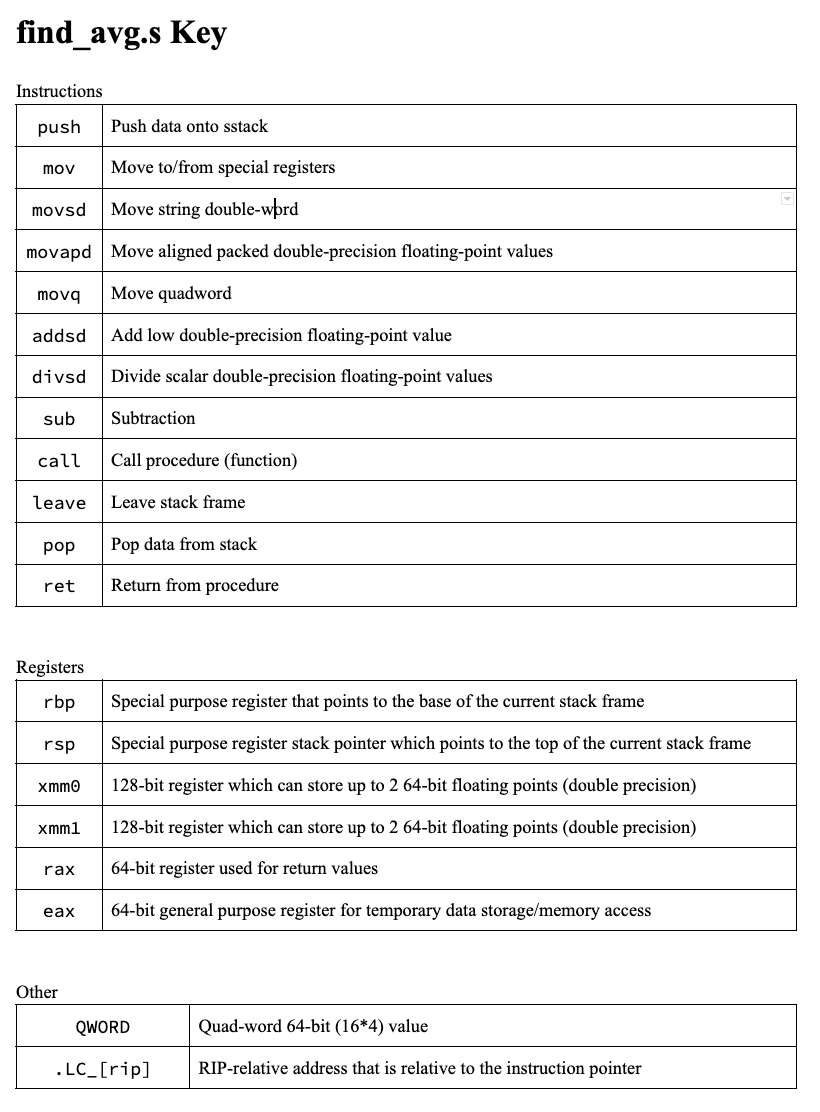
\includegraphics[width=.75\textwidth]{Images/find_avg.s_key.png}
\cite{AG}

\bigskip\noindent
As we can see, the assembly code is much more complicated than the WebAssembly. This is because there is much more involvement with the hardware since gcc is compiled to run on a local machine, and not the web. In the above key, we can view all of the different kinds of registers that are required for \verb|find_avg.cc|. \verb|rbp|, for example, points to the base of the current stack frame, and \verb|xmm0| is designed to store 64-bit doubles. Keep in mind that these respective registers and instructions are specific to the architecture of x86 processors. There are also a variety of instructions that aren't found in the WebAssembly code. There are no \verb|mov| instructions in WebAssembly, and this is because it does not have to worry about local hardware. The stack also seems much simpler when viewing WebAssembly code because it does not have to push and pop at the hardware level with registers.


\section{Conclusion}\label{conclusions}

\medskip\noindent
As shown, studying the assembly language and especially WebAssembly behind individual is good for getting an understand of what the computer, or web service, needs in order to run programs. WebAssembly is great for viewing programs on the stack, and comparing the stack structure to the abstract syntax tree. Traditional assembly language, on the other hand, is better for getting an understanding of how the code eventually is processed by the computer hardware, specific to individual processor types. Even though it is not as practical as WebAssembly for understanding abstract syntax, it can be very interesting to see where software and hardware meet. Overall, there is and always will be an abundance of material that can be learned from low-level languages.

\begin{thebibliography}{99}
\bibitem[PL]{PL} \href{https://github.com/alexhkurz/compiler-construction-2022/}{Compiler Construction 2022}, Alexander Kurz, 2022.

\bibitem[AC]{AC} \href{https://blog.holbertonschool.com/hack-virtual-memory-stack-registers-assembly-code/}{Assembly Code \& the Stack}, Julien Barbier, 2017.

\bibitem[AG]{AG} \href{https://www.cs.virginia.edu/~evans/cs216/guides/x86.html}{x86 Assembly Guide}, University of Virginia Computer Science, 2006.

\bibitem[WA]{WA} \href{https://developer.mozilla.org/en-US/docs/WebAssembly}{WebAssembly}, MDN Web Docs, 2022.

\bibitem[AL]{AL} \href{https://www.investopedia.com/terms/a/assembly-language.asp}{Assembly Language}, Jason Fernando, 2020.

\bibitem[AS]{AS} \href{https://www.inf.ed.ac.uk/teaching/courses/ct/17-18/slides/7-ast.pdf}{Abstract Syntax}, Christophe Dubach, 2017.


\end{thebibliography}

\end{document}
